\chapter{Control}
\label{ch:control}
\head{This chapter describes the selected strategy from
	chapter~\vref{ch:selformctrl} in more detail, describing the exact
algorithm.}




% This is a summary of how they use Potential Fields in "UAV Formation Flight using 3D Potential Field"
\section{One Approach for Potential Fields}
In the following approach a potential field is generated for each
agent including obstacles, formation span, desired, and actual
position.  It will be a combination of virtual leader and potential
field. The principle generates a potential field to keep the formation
and that field is moved around as a virtual leader. When the virtual
leader is moved around it results in a deflection of the desired
position and causes the affected agents to get back into position. The
positions of the agents in the field is given individually to the
specific agents relative to the virtual leader. The approach generates
a single resulting vector for each agent which is used to guide the
agent. The potential field for each agent is generated from four
components:
\begin{align}
\tilde{F}_i^{tot} = F_{vl}+F_{ij}^{tot}+F_{ca}^{tot}+F_{oa}^{tot}
\end{align}
where:
\begin{ffk}
\firmlist%
\item[$F_{vl}$] virtual leader force
\item[$F_{ij}^{tot}$] inter-agent forces
\item[$F_{ca}^{tot}$] agent-agent collision avoidance forces
\item[$F_{oa}^{tot}$] agent-obstacle collision avoidance forces
\end{ffk}

\subsubsection{Virtual Leader, $F_{vl}$}
The virtual leader is an anchor of each formation, the \ac{FRP}, and
controls the movement of this. This movement can either be given as a
full trajectory of as a set of way points. The local virtual leader's
contribution to the field is defined as:
\begin{align}
F_{vl} &= K_{vl}(p_{vl}^n-p_i^n-[p_{vl}^n-p_{i0}^n])\\
&= K_{vl}(d_i-d_{i0})
\end{align}
$K_{vl}$ is a tuning parameter. $p_{vl}$ is position of the virtual
leader, $p_i$ is position of agent $i$, $p_{i0}$ is desired position
of agent $i$ and the $d$ is a shorter notation for the distances in
between. The virtual leader component guides the agents directly to
their desired positions relative to the virtual leader.

\subsubsection{Inter Vehicle Influence, $F_{ij}$}
This is the contribution of other vehicles to the potential field,
which is expressed as:
\begin{align}
F_{ij} &= K_{ij}(p_{j}^n-p_i^n-[p_{j0}^n-p_{i0}^n])\\
&= K_{ij}(d_{ij}-d_{ij0})
\end{align}
Similar to previously the $p$s are positions, $K_{ij}$ is a tuning
parameter and $d$ is a shorter notation for the distances in between.
This component preserves the formation by affecting the agents to keep
their respective desired distances among themselves. Hence the
weighting on each goal can be adjusted by $K_{vl}$ and $K_{ij}$ a
weighting that causes the agents to follow the virtual leader or to
preserve their desired formation.  In a swarm of $N$ agents the total
field for agent $i$ given by:
\begin{align}
F_{ij}^{tot} = \sum\limits_{j=1}^NF_{ij}(i,j) \text{ for } j\neq i
\end{align}

\subsubsection{Collision Avoidance, $F_{ca}$}
The collision avoidance takes effect when the agents get closer than a
pre defined distance of each other. It generates an additional field
component for the vehicle $i$ which points away from the entering
agent causing the agents to move away from each other. To ensure the
avoidance the component converges towards infinity in the centre of
the $i$'th agent. The $F_{ca}$ is expressed as:
\begin{align}
    F_{ca}^{ij}= 
\begin{cases}
		\left(
    \frac{K_{ca}r}{||d_{ij}||}-K_{ca}
		\right)
		\frac{\mathbf{d}_{ji}}{||\mathbf{d}_{ji}||}
		,& \text{for } ||d_{ij}||<r\\
    0,              & \text{otherwise}
\end{cases}
\end{align}
where $K_{ca}$ is a tuning parameter. $r$ is the safety radius for
collision and $d_{ij}$ is the distance between the individual agents.
The collision avoidance can be expressed in a total term of the
collision avoidance:
\begin{align}
F_{ca}^{tot} = \sum\limits_{j=1}^NF_{ca}^{ij} \text{ for } i\neq j
\end{align}

\subsubsection{Obstacle Avoidance, $F_{oa}$}
The same principle as for collision avoidance can be applied to
obstacle avoidance. Now each obstacle needs to be handled as an agent,
which will make the same result, but the reference is a little
different:
\todo{describe why the oa is different from the ca}
\begin{align}
    F_{oa}^{ik}= 
\begin{cases}
    \left( \frac{K_{oa}}{||d_{ki}||}-\frac{K_{oa}}{r}\right)
		\frac{\mathbf{d}_{{ki}}}{||\mathbf{d}_{ki}||},& \text{for } ||\mathbf{d}_{ki}||<r\\
    0,              & \text{otherwise}
\end{cases}
\end{align}
where $k$ denotes the counter for obstacles instead of other agents.
$K_{oa}$ is also a tuning parameter for the obstacle avoidance.
$d_{ki}$ is the vector between an agent and the obstacle, which in a
total term is summed up as:
\begin{align}
F_{oa}^{tot} = \sum\limits_{k=1}^MF_{oa}^{ik} \text{ for } i\neq k
\end{align}
Here $d_{ki}$ represents one of the $M$ place vectors which has the
effect of a detected obstacle.  The distance $r$ can be determined
dynamically depending on the velocity of the agent:
\begin{align}
r = r^{min} + K_r||\dot{p^n}||
\end{align}

\subsubsection{Potential field}
Now these forces was summed together to get
$\tilde{F}_i^{tot}$, that was just an intermediate vector, which needs
to be limited in a way, because this describes the speed the agents
can move with.

which gives the magnitude and direction of the
potential field for vehicle $i$ at its current position. As the
potential field does not need to expand to infinity it is reasonable
to define a maximum amplitude for the vector, while still keeping its
direction:
\todo{Denne afsluttende subsubsection er underligt formuleret, husk
det med tilden, og sikkert også hvordan vi jegner p\_r}
\begin{align}
	F_i^{tot} = \min\{\,\,\,||\tilde{F}_i^{tot}||\,\,\,,\,\,F_{max}\,\,\,\}\frac{\tilde{F}_i^{tot}}{||\tilde{F}_i^{tot}||}
\end{align}


\section{The Potential Field Strategy}
The theory of potential fields are implemented with the strategy
proposed in section \ref{sc:potential-fields}. The potential field is
generated for each individual agent at every update step to make the
formation move and converge to a specified formation and position. The
field is generated based on forces acting in a overlying potential
field structure where one force converges the agent to a desired
position, a force attracting the agent to obtain the desired formation
along the trajectory, a force repelling the agent from other agents if
their distance is too small and finally a force repelling the agents
from static objects. The latter two can seem the same, but the
repelling force will be larger for the agent-agent force due to the
fact that two agents could have course directly toward each other and
a more aggressive avoidance can be needed.

To be able to generate and simulate the potential field then
implementation needs to be generic. First it was developed with one
agent that needs to converge to a desired position and afterwards were
other agents added as obstacles and some static objects were added in
extend. From these obstacles it can be seen that a single agent is
able to converge to a position which makes it possible to expand such
that more agents can converge into formation with reference from
either a virtual leader or from each other. This will solve the
formation coordination task, where the following task will be the
group coordination task. The group coordination task has the goal to
move the formation around, which here will be done by making the
virtual leader, or an actual leader of the formation, follow a
trajectory specified. This will make the other agents follow this
leader and withhold their formation on the trajectory.
\begin{figure}[htbp]
  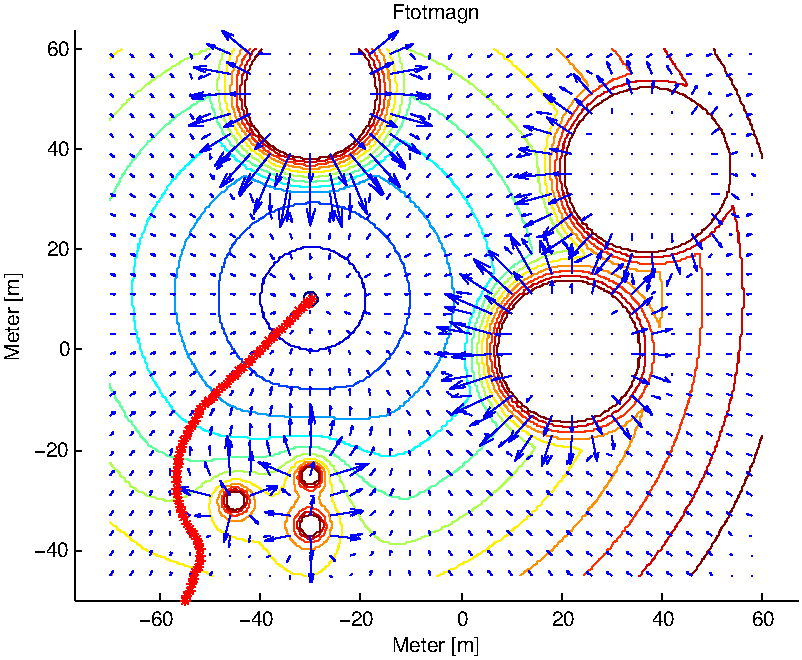
\includegraphics[width=0.9\textwidth]{fig/ftotmagnfigpdf1}
  \caption{Plot of one agent's trajectory with a desired position with obstacles to avoid}
  \label{fig:potfieldagenti}
\end{figure}
A plot for a total potential reference field for a single agent can be
seen on figure \ref{fig:potfieldagenti}. The red line made of crosses
is the trajectory that one single agent will follow, if the obstacles
to avoid in the plot are static. In the plot every object, either
another agent or an object, are kept static. So it shows how the
trajectory will be in one single time step. This will change in the
next time step if the other agents also move in the potential field.
The agent avoids obstacles on the way, where it can be seen that it
does not get into the safety radius of the obstacles. In this specific
plot is a safety radius ($r$) of $20$m chosen, such that the distance
from agent $p_i$ (The red trajectory) to any obstacle always will be
larger than $20$m.

The gains $K_{ca}$ and $K_{oa}$ are chosen equally to a constant as
240. If this gain is chosen smaller it will result in that the agents
are more allowed to approach the obstacles and get a little within the
radius, but then afterwards getting repelled from the object. It
corresponds to the gradient at the radius and how steep this is.

The same algorithm is applied where agent $i$ avoids other agents, agent $j$, $j+1$. This can be seen on figure \ref{fig:avoidagent}.
\begin{figure}[htbp]
  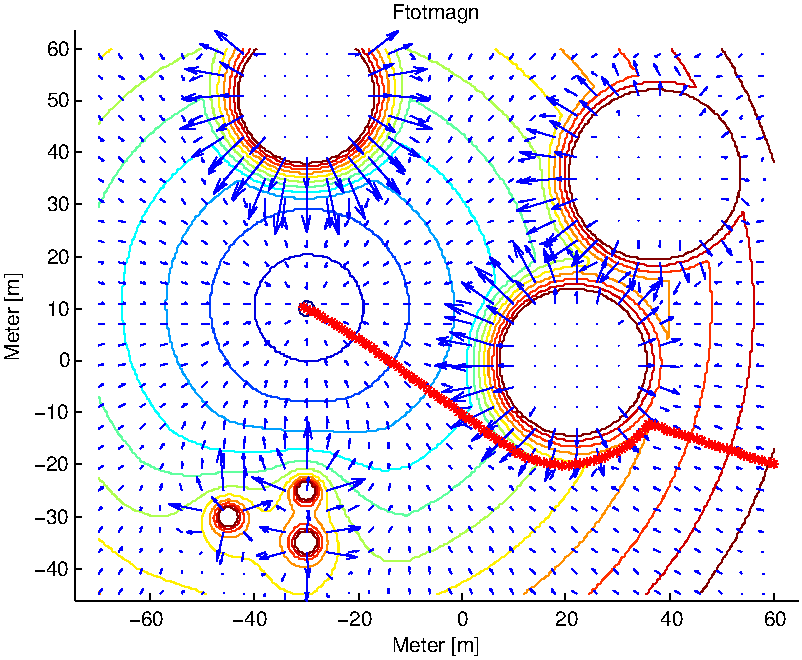
\includegraphics[width=0.9\textwidth]{fig/ftotmagnfigpdf}
  \caption{Agent $i$ avoids agent $j$ and converges to the minima at the virtual leader}
  \label{fig:avoidagent}
\end{figure}
Agent $i$ takes a direct course toward the virtual leader but meets
another agent as an obstacle. Agent $i$ moves on the boarder of agent
$j$ with the defined safety radius and afterwards diverges from agent
$j$ towards the virtual leader. This is all done by following the
lowest gradient at all times.

The gain of $K_{ij}$ is not to be interpret from figure
\ref{fig:potfieldagenti}. $K_{ij}$ is the gain to the force that
attracts the agents together by minimizing the distance in between
them. By doing this the agents will get faster into the desired
formation. The gain $K_{vl}$ does at some point the opposite. This
gain adjusts the weighting of how fixated the agents should be to
converge to the desired position. If this gain is relatively larger
than $K_{ij}$ then the agents will converge directly to their position
around the virtual leader and not converge to the desired formation on
the way. This implies that the scaling between $K_{vl}$ and $K_{ij}$
controls if the formation should converge to the desired formation on
the way to the desired position, or if agent $i$ should only have the
desired position in focus.

The grid in which the potential field is generated are limited with a
certain resolution while simulating the agents movement. This reduces
the directions of where the agents can move, which will not arise a
problem on the same level when implemented in reality. In the
simulation environment it reduces the resolution such that a single
field in the grid contains one value of magnitude of the potential
field, which makes the basis of a certain gradient to the field. The
agents are following the implementation of the steepest decent. This
generates a gradient towards the steepest decent, which the agent
tracks. The analogy can be seen as a bowl, or sphere in this case,
where a ball will converge towards the lowest point in the direction
of the minimum gradient.

The method of applying the grid with magnitude of the potential field
arises the problem with resolution, but also a problem that makes the
'corners' of the grid around the agent to be more likely to have the
steepest decent. This is seen as if the agent is placed in the middle
of a 3-by-3 matrix, and have eight placements around it. This problem
has been expanded with a solution such that a certain radius in the
potential field around an agent will be checked. The value at the
radius around the agent can be checked, and due to the equal distance
to every point, these will be weighted equally with respect to their
value. This makes in principle the possibility to make the agent go in
all directions which will be closer to the reality. When testing the
two methods against each other it is clear that the first proposed
with the grid structure did not have the same mobility thus not
preferable in simulations though it is simpler.
\todo{This section is not really clear}

Another problem that can become crucial arises when two agents or two
objects are within the radius of each other. This will result in a
local minima in the potential field between those objects. This will
create a small local minima in between these agents or objects. If an
agent converges toward this minima they cannot get out again. The
problem can be seen on figure \ref{fig:roevproblem}. The gains here
are chosen exactly the same as in figure \ref{fig:potfieldagenti}.
\begin{figure}[htbp]
  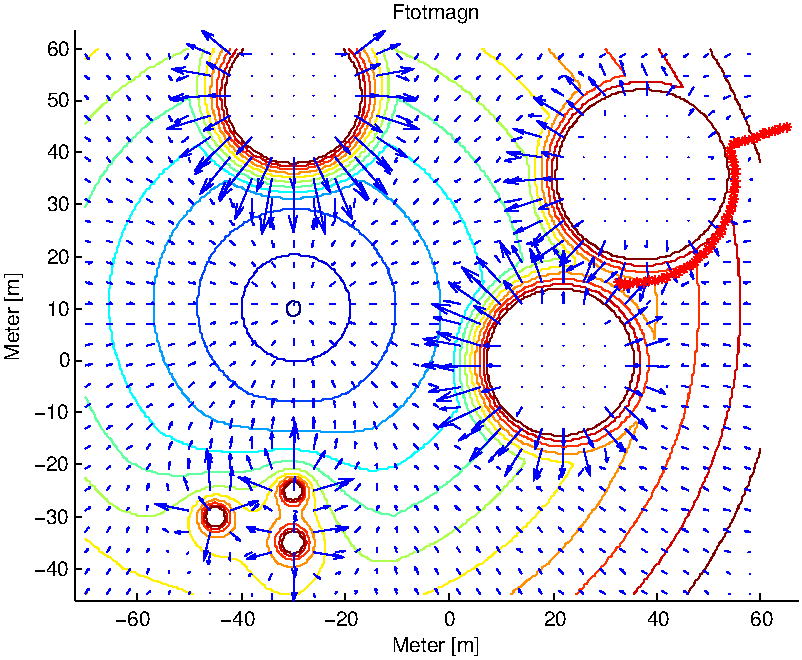
\includegraphics[width=0.9\textwidth]{fig/ftotmagnfigpdf3}
	\caption{An agent gets stuck due to a local minima between two other
	agents. The agent cannot get out of this minima unless the other two
	agents makes the space for the agent to pass through}
  \label{fig:roevproblem}
\end{figure}
The scenario on figure \ref{fig:roevproblem} has the following steps.
The agent $i$ moves in the direction of the steepest decent. Then it
gets to the border of another agent where it cannot go through thus
starts to go around this agent. The problem arises when agent $i$
reaches another agent on the way where it now has reached a local
minima. Now the steepest gradient will point at the position where the
agent already is thus making it think it has reached the end point.
Solutions to this problem can be formulated in different ways. One
solution could be to cluster the two objects together and instead of
making their potential field individually, then combine those together
and make an ellipsoid or even a circle formed obstacle of those
objects. This will ensure that the local minima disappears thus not
making an agent get stuck between those objects. Another solution is
to make an exception handler that can tell if agent $i$ has reached
the desired position. If it has not reached its end point, and the
position is constant on the same placement, it perturbs the desired
position of the agent until the direction of the steepest decent
changes more than a predefined value. This will mean that the agent is out of the local minima and can continue on the trajectory.
The solution of clustering the objects, that are too close, can be seen on figure \ref{fig:solroevproblem}.
\begin{figure}[htbp]
  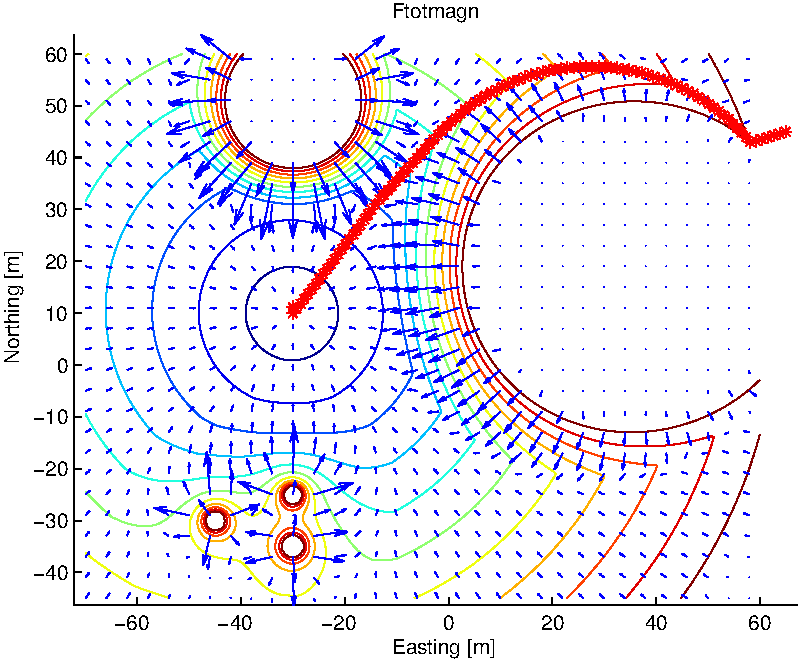
\includegraphics[width=0.9\textwidth]{fig/ftotmagnfigpdf4}
  \caption{An agent that before was stuck now does not get into a local minima close to the agents, as it now sees the two other agents as one larger agent.}
  \label{fig:solroevproblem}
\end{figure}
Here the first solution is applied where the two agetns, that were too close to each other, have been clustered into one, seen from the $i$'th agent. Now the local minima between the agents have been neglected and the $i$'th agent can generate its trajectory around the agents and continue to the endpoint of the potential field. The algorithm checks if the distances between the agents are lower that $2 \cdot r$. If this is the case it means that the $i$'th agent cannot generate a trajectory in between these agents, which can lead to a local minima. Therefore is the agents that are too close combined into one by generating the middle point between their positions and generating a new radius. This makes a larger circle where the two agents are in the subset. This cricle will be larger depending on the wanted safety radius thus rises the need to recheck the potential field again after have generated a new combined agent. If the radius of the new agent places it close to one of the single agents, these also might need to cluster. Thus the algorithm needs to run untill no distances between agents are $< 2 \cdot r$.
The algorithm generating this combined agent can be seen in pseudo code in algortihm \ref{al:clusteragents}.
\begin{algorithm}[H]
  \KwData{clustering of agents}
  initialization\;
  \If{$||\mathbf{p}_i , \mathbf{p}_j|| < 2 \cdot r$}{
  $\mathbf{p}_{j,new} \gets \text{mid point between}\ \mathbf{p}_i\ \text{and}\ \mathbf{p}_j$\\
  $r_{new} \gets \text{calc new r for}\ \mathbf{p}_{j,new}$\\
  delete $\mathbf{p}_i\ \text{and}\ \mathbf{p}_j \text{with}\ \mathbf{p}_{j,new}$
  }
  \caption{This pseudo code describes how agents that are too close to eachother are getting clustered and seen as one. The algorithm can also be applied for obstacles in the potential field.}
  \label{al:clusteragents}
\end{algorithm}
Firstly every distance between the agents are checked if it is lower than $2 \cdot r$. If the distance is lower, a new coordinate set needs to be calculated. The coordinates for the $\mathbf{p}_{j,new}$ is generated to the middle value of the two points
\begin{align}
\mathbf{p}_{j,new} = \frac{\mathbf{p}_i + \mathbf{p}_j}{2}
\end{align}
and afterwards can the new radius for $\mathbf{p}_{j,new}$ be found from
\begin{align}
r_{new} = \frac{||\mathbf{p}_i , \mathbf{p}_j||}{2} + r
\end{align}
The $r_{new}$ is visualized on figure \ref{fig:rnew}
\begin{figure}[htbp]
\centering
\includesvg{rnew}
\caption{Illustration of two agents close to each other clustering into one new agent. The two original agents, $i$ and $j$ are coloured in black and the new clustered object are coloured in green. The distance between $i$ and $j$ is coloured in red.}
\label{fig:rnew}
\end{figure}
This shows the relation between the normal safety radius and the new radius defined for the new clustered agent.

In the end this results in that the every agent needs a magnitude and
a direction of which they should move. This will be given depending on
the total environment where the agents are manoeuvring, and will be assigned by the gradient vector. When applying
this formation strategy a collision free movement is guaranteed which
is one of the more critical criteria to be fulfilled. \todo{Det her
skal der nok skrives lidt matematik om som viser det, eller en god
forklaring. Men dog er det jo en naturlig del af pot field.}


\subsection{Adding the Dynamics for Simulation}
\todo{Describe the block diagram connecting the potential field calculations,
an analogy to the wp\_gen script for the path follower.}

Describe the behaviour when a boat gets stuck in a local minima.

\begin{figure}[htbp]
\centering
\includesvg{potentialfield_block}
\caption{Block diagram showing the iteration process of using the
potential fields for computation of the input vector}
\label{fig:potentialfield_block}
\end{figure}

The potential field control system consists of multiple elements
as seen with the e flow is illustrated on the block diagram on
figure~\vref{fig:potentialfield_block}.

Part og this flow can be computed by the $i$'th ship themselves.

The implementation of this is tested in matlab, using the m-files;

potfield.m, pathgen.m, shipcontroller.m, simaauship.m

The simulation algorithm for the multiship potential field should keep
in mind that shall save the timeseries for the ship states, the
control inputs and the local reference trajectory for the $i$'th ship.

Ignoring the initialization of all the variables, the outer loop
guidance navigation and control algorithm using potential fields are
as follows.

The \ac{GNC} works by an array of mission specific way points given,
usually computed from a desired area used to create a lawnmower
pattern described in chapter~\vref{ch:pathgen} describing the path
generation.

\paragraph{Global Trajectory Generation}
Then different methods can be used to steer ships after this
trajectory. The simplest is the usual heading autopilot, which will
just steer the reading of the ship to the course angle to the
way point. Or more elaborate, ways is the use of the way points as
linesegments that the ship should follow. This is implemented with a
\ac{LOS} algorithm. This algorithm, can work, but it is too simple to
include obstacle or inter vehicle collisions. A way proposed to solve
this issue is to use the concept of potential fields.

\paragraph{Potential Field}
The potential field itself is merely some functions describing the
repulsive and repelling forces between points of interest in the map.
These points of interest are all objects that matters for the
navigation, that is all ships, the anchor point (virtual leader) of
the formation, and other point obstables. This using the methodology
described in the paper \citep{UAVff3dpf}.

The potential field is used in an iterative algorithm which can
calculate the direction (from the $i$'th boat to the desired position
spaned by a potential field defining the formation.

\paragraph{Local Trajectory Generation}
In the end, a reference path is calculated by the means of the
previous position and the result from the potential field
solver. It is calculated as the paper presents, \citep[eq.
48]{UAVff3dpf}.

\begin{align}
	\mathbf{p}_{i,r}^n = \mathbf{p}_i^n + \mathbf{F}_i ^\text{tot}
\end{align}

This is passed to the ships inner control loop.

When the trajectory is generated from a series of way points, which is
not ordered as a series of equidistant way points, it means that some
handling of when or how to update the position of the virtual leader
is needed.

For example; in the case, where the way points are far from each
other, it is still desired to make the virtual leader trajectory
converge the line between these two way points, kind of like the
\ac{LOS} guidance. Earlier a path following algorithm using a \ac{LOS}
principle was used, to calculate a course angle to a point projected
into the line between two way points with a specified lookahead
distance. The projection with the lookahead ensures convergence to the
line. But in the case of controlling the virtual leader, it is not
necessary to calculate the course angle from the virtual leader to the
projected point, because this is only a virtual anchor of the
formation, hence this only specifies where the geometry of the
formation is calculated from. 

For the inner loop, a heading based \ac{LOS} method can still be used,
but this should be calculated for every ship, with each their
reference position $\mathbf{p}_{i,r}$.

\begin{algorithm}[H]
	\KwData{track as global mission trajectory as way points}
	initialization\;
	\While{$m <=$ length of track}{
		\For{every $i$-th boat}{
			\If{formation is ok}{
				\If{$p_{vl}$ is inside the way point acceptance radius of the
				track}{
					$m \gets m + 1$\; 
					$p_{vl} \gets$ \textsl{LOS}$(\ p_{vl}\ ,\ $track($m$)\ )\;
				}
			}
			$(\ p_{d,i}\ ,\ F_{\text{tot},i}\ ) \gets $  \textsl{pathgen}(\ $p_i$\ ,\ $p0_i$\ )\;
			$p_{r,i} \gets p_i + F_{\text{tot},i}$\;
			$\psi_{d,i} \gets $ heading from $p_i$ to $p_d$\;
			$u_i \gets $ \textsl{controller}(\ $\psi_d$\ )\;
			\textsl{send input $u$ to ship}\;
			$x_i \gets $ \textsl{sense ship states}\;
			$p_i \gets $ position of $x_i$\; 
		}
	}
	\caption{This pseudo code describes how the potential field is used
	for each boat to calculate the reference for the inner controller
	for every boat at every time step. Every iteration in the while loop
	is a time step.\vspace{6pt}}
	\label{al:potfield}
\end{algorithm}

The algorithm~\vref{al:potfield} describes how the potential field
strategy can be simulated, were each iteration of the while loop is a
time step, which means that the control will continue until the
formation has reached the way point acceptance radius of the track.
This is to ensure that the formation anchor do not move forward if the
ships are not properly in formation. This is analogous with the group
coordination task as defined by \citep{thorvaldsen}, and described in
section~\ref{sc:initialisation}.

For the real implementation in \ac{ROS}'s node structure, only loop
inside the for every boat should be a node, such that there could be
$i$ instances of this node, each representing one boat. 




\todo{Describe how the dynamics will affect the trajectory.}
